\documentclass[11pt,a4paper]{article}
\usepackage[utf8]{inputenc}
\usepackage{geometry}
\geometry{margin=2.5cm}
\usepackage{graphicx}
\usepackage{listings}
\usepackage{xcolor}
\usepackage{hyperref}
\usepackage{amsmath}

\title{\textbf{Dokumentation: Gesichtserkennung mit Faster R-CNN und MobileNet v3}}
\author{Angewandte Modellierung – Projektarbeit}
\date{\today}

\definecolor{codegray}{rgb}{0.95,0.95,0.95}
\lstset{
backgroundcolor=\color{codegray},
basicstyle=\ttfamily\small,
frame=single,
breaklines=true,
language=Python,
showstringspaces=false
}

\begin{document}

\maketitle

\tableofcontents
\newpage



\section{Motivation}
Vision AI interessiert mich schon sieht ein paar Jahren angefangen synthetischen Frames(NVIDIA RTX) und FSD in 2019 und 2022. Für dieses Projekt hat mich vor allem interessiert wie gut man heute Vision AI lokal trainieren und benutzen kann. Als simples Beispiel habe ich die Face recognition gewählt.

\section{Dataset}
Es gibt viele Datensets für Face recognition bei der lokalen Nutzung muss man aber abwägen wie viele Daten sowohl in den Speicher passen und wie lange man trainieren kann. Deshalb habe ich mich für ein relativ kleines Datenset entschieden das aus dem WIDER Dataset extrahiert wurde, WIDER ist ein event Dataset, WIDER Face.

\subsection{WIDER Face}
Das WIDER Face Dataset umfasst insgesamt 32.203 Bilder und über 393.703 Gesichtsexemplare, verteilt auf Training, Validierung und Test. Es zeichnet sich durch hohe Variabilität in Szene, Beleuchtung, Auflösung und Gesichtsausdruck aus.

\subsection{Annotations}
Die Ground-Truth-Anmerkungen liegen in Textdateien vor, jeweils für Trainings- und Validierungs-Splits. Jede Bild-Datei wird durch mehrere Zeilen mit Bounding-Box-Koordinaten und Zusatzattributen beschrieben:
\begin{itemize}
\item x y w h: linke obere Ecke (x,y) sowie Breite und Höhe der Box
\item blur, expression, illumination, invalid, occlusion, pose: qualitative Attribute (0/1), wobei invalid=1 das gesamte Gesicht markiert und zur Filterung dient.
\end{itemize}
Eine Python Funktion load\_widerface\_annotation filtert ungültige Einträge und wandelt (x, y, w, h) in zwei Eckpunkte (x1, y1, x2, y2) um. Jedes Gesicht erhält das Label 1 (Gesicht), Hintergrund 0.

\section{Modell und Aufbau}
\subsection{Faster R-CNN}
Faster R-CNN ist eine zweistufige Objekterkennungsarchitektur:
\begin{enumerate}
\item Region Proposal Network (RPN) generiert mögliche Objektregionen.
\item Klassifikations- und Box-Regression-Head verfeinert diese Regionen.
\end{enumerate}
Die Verknüpfung beider Schritte macht Faster R-CNN effizienter als frühere RCNN-Varianten.

\subsection{MobileNet v3 large FPN}
Als Backbone dient MobileNet v3 large mit Feature Pyramid Network (FPN):
\begin{itemize}
\item MobileNet v3: leichtgewichtig, geringe Latenz, tauglich für Echtzeit‑Anwendungen.
\item FPN: kombiniert Merkmale aus verschiedenen Skalen, um Objekte unterschiedlicher Größe robust zu erkennen.
\end{itemize}
Der Klassifikator-Head wurde angepasst: statt der Standard-Labels (z. B. COCO-Klassen) wurde nur zwischen Gesicht und Hintergrund unterschieden (num\_classes=2).

\section{Pipeline}
\subsection{Daten laden}
\begin{lstlisting}
train_records = load_widerface_annotation(train_txt, train_images)
val_records   = load_widerface_annotation(val_txt, val_images)

train_ds = ObjectDetectionDataset(train_records, transforms=get_transforms(train=True))
val_ds   = ObjectDetectionDataset(val_records, transforms=get_transforms(train=False))
\end{lstlisting}

\subsection{Training}
\begin{itemize}
\item Epochen: 10
\item durch alle Trainings Bilder iterieren und die Loss Funktion berechnen
\item dann noch einen Validierungsdurchlauf und auch auf den Validierungsdaten die Loss Funktion berechnen
\end{itemize}
Trainingsschleife:
(\href{https://github.com/7hands/Angewandte-Modellierung-25-Colmant/blob/main/Vortrag_Projeckt/image_detect.py}{Trainings Code (200-216)})
\begin{lstlisting}
for epoch in range(num_epochs):
    # Training
    model.train()
    train_loss = 0.0
    for imgs, targets in train_loader:
        imgs = [img.to(device) for img in imgs]
        targs = [{k: v.to(device) for k, v in t.items()} for t in targets]
        loss_dict = model(imgs, targs)
        losses = sum(loss for loss in loss_dict.values())
        optimizer.zero_grad(); losses.backward(); optimizer.step()
        train_loss += losses.item()
    lr_scheduler.step()
    avg_train = train_loss / len(train_loader)

    # Validation
    val_loss = 0.0
    with torch.no_grad():
        for imgs, targets in val_loader:
            imgs = [img.to(device) for img in imgs]
            targs = [{k: v.to(device) for k, v in t.items()} for t in targets]
            loss_dict = model(imgs, targs)
            val_loss += sum(loss for loss in loss_dict.values()).item()
    avg_val = val_loss / len(val_loader)
\end{lstlisting}

\subsection{Gewichte speichern}
Nach dem Training werden die Gewichte mit torch.save(model.state\_dict(), ...) in checkpoints/ gesichert.

\subsection{Inference}
Das Inferenz-Skript lädt die gespeicherten Gewichte, führt Vorhersagen auf neuen Bildern durch und speichert Visualisierungen mit Bounding-Boxen:
\begin{lstlisting}
def run_inference(model, image_paths, output_dir: Path, device, threshold: float = DEFAULT_THRESHOLD):
    output_dir = output_dir.resolve()
    output_dir.mkdir(parents=True, exist_ok=True)
    print(f"Saving results to: {output_dir}")
    to_tensor = ToTensor()

    for img_path in image_paths:
        img_path = Path(img_path).resolve()
        if not img_path.is_file():
            print(f"[WARN] Datei nicht gefunden: {img_path}")
            continue
        img = Image.open(img_path).convert("RGB")
        img_tensor = to_tensor(img).to(device)
        with torch.no_grad():
            outputs = model([img_tensor])[0]

        boxes = outputs['boxes']
        scores = outputs['scores']
        labels = outputs['labels']
        keep = scores >= threshold

        img_boxes = draw_bounding_boxes(
            (img_tensor * 255).to(torch.uint8),
            boxes[keep],
            labels=[str(int(l.item())) for l in labels[keep]],
            width=2
        )

        save_path = output_dir / img_path.name
        from torchvision.transforms import ToPILImage
        ToPILImage()(img_boxes).save(save_path)
        if save_path.is_file():
            print(f"Saved inference result to {save_path}")
        else:
            print(f"[ERROR] Konnte Datei nicht speichern: {save_path}")
model = load_model(checkpoint_path, device)
run_inference(model, image_paths, output_dir, device, threshold=0.5)
\end{lstlisting}
Dabei werden nur Vorhersagen mit Score $\geq$ Threshold gezeichnet.
\newpage
\section{Ergebnisse}
Positiv Beispiele:
\begin{figure}[h!]
\centering
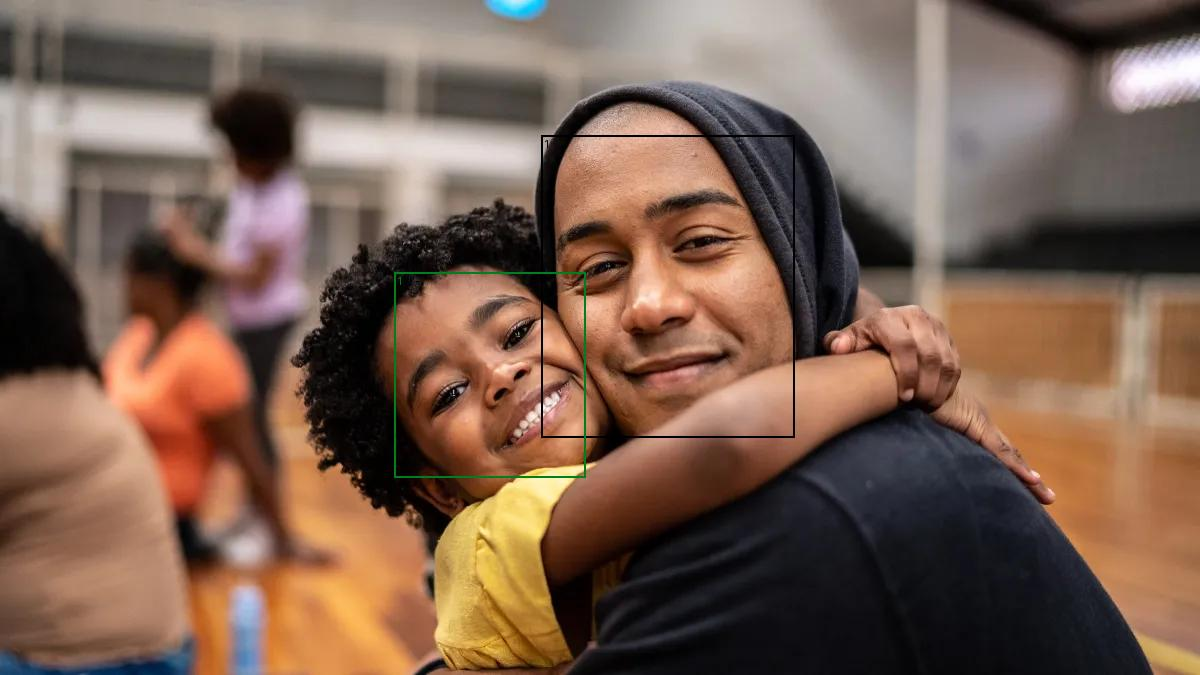
\includegraphics[width=0.45\textwidth]{../inference_results/people.jpg}
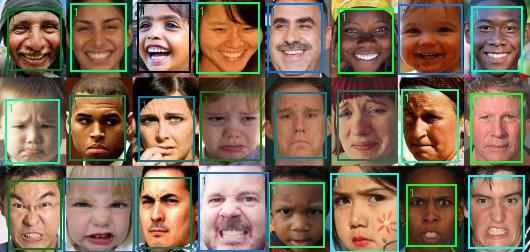
\includegraphics[width=0.45\textwidth]{../inference_results/common-emotions.jpg}
\caption{Beispielhafte Inferenz-Ergebnisse auf eigenen Bildern.}
\end{figure}
\begin{figure}[h!]
\centering
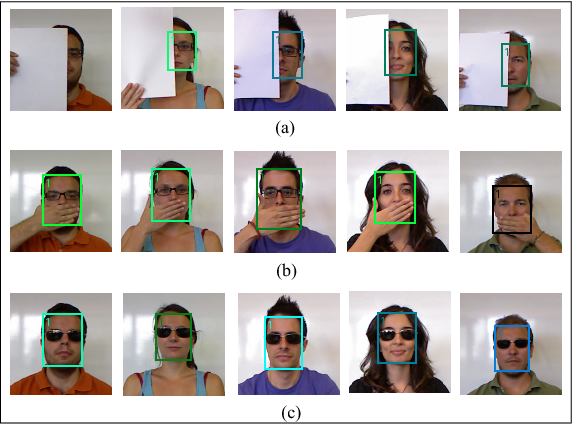
\includegraphics[width=0.45\textwidth]{../inference_results/ocluded.png}
\caption{Besonders beindruckend auch Bilder auf dem die Gesichter nicht richtig erkennbar sind können in vielen Fällen erkannt werden.}
\end{figure}\\
Negativ Beispiel:
\begin{figure}[h!]
\centering
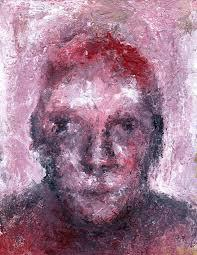
\includegraphics[width=0.25\textwidth]{../inference_results/foggy-painting.jpg}
\caption{in dem impressionistischen Portrait wurde kein Gesicht erkannt.}
\end{figure}

Schwierige Szenen (starke Verdeckung, schwache Beleuchtung, keine Fotos) zeigten gelegentlich Fehl- oder Nicht-Erkennungen.


Quantitativ erreicht das Model nach 10 Epochen auf einem Validierungs-Subset einen Loss über alle Validierungsbilder von 0.33.

\section{Fazit}
Das Projekt zeigt, dass Gesichtserkennung lokal mit Fast R-CNN und MobileNet v3 möglich und verhältnismäßig effizient ist. Trotz begrenzter Datenmenge und kurzer Trainingszeit wurden zufriedenstellende Erkennungsraten erzielt. Für zukünftige Arbeiten sind folgende Verbesserungen denkbar:
\begin{itemize}
\item Erweiterung des Datensets (z. zusätzliche Variationen, Augmentationen)
\item Feintuning weiterer Backbones (z. z. B. ResNet, EfficientNet)
\item Optimierung der Inferenzgeschwindigkeit (Quantisierung, TensorRT)
\end{itemize}

\section{Quellen}
Data Set auf Kaggle: \url{https://www.kaggle.com/datasets/mksaad/wider-face-a-face-detection-benchmark/data}

\begin{thebibliography}{9}
\bibitem{wider} Yang, Shuo, et al. "WIDER FACE: A Face Detection Benchmark." \emph{Proceedings of the IEEE Conference on Computer Vision and Pattern Recognition}, 2016.

\bibitem{fasterrcnn} Ren, Shaoqing, et al. "Faster R-CNN: Towards Real-Time Object Detection with Region Proposal Networks." \emph{IEEE Trans. on Pattern Analysis and Machine Intelligence}, 2017.

\bibitem{mobilenetv3} Howard, Andrew, et al. "Searching for MobileNetV3." \emph{IEEE International Conference on Computer Vision}, 2019.

\bibitem{torchvision} PyTorch Team. "Torchvision: Models for PyTorch." \url{https://pytorch.org/vision/stable/models.html}
\end{thebibliography}

\end{document}






